\chapter{Computer networks}\label{chapter:computer-networks}

\section{Network types}

\section{Implementation}

\subsection{Protocols}

\subsection{Services}


\section{OSI layers}

\subsection{Physical layer}
\subsection{Data link layer}
\subsection{Network layer}
\subsection{Transport layer}
\subsection{Session layer}
\subsection{Presentation layer}
\subsection{Application layer}

In what follows we'll briefly discuss the web platform. Most internet users will navigate the web using a web browser. A web browser is a piece of software that displays HTML, and executes JavaScript. It allows the user to interact with multiple sites at the same time, and handle user interface and network events.

Browsers also offer a powerful API to scripts:
\begin{itemize}
	\item Inspecting / modifying the page;
	\item Inspecting / modifying page metadata, e.g. Cookies;
	\item Sending / receiving HTTP (XMLHttpRequest API);
	\item Event handling.
\end{itemize}

The following paragraphs take a closer look at the typical elements that are used when navigating to a web page. These include the URL to find the resource, a stateless communication protocol to transer the application data and ways to introduce state, and a markup language and scripting langauge to view and run the web page/application.


\subsection{Uniform Resource Locator}

When a user wishes to access an online web page via his/her browser, he/she will enter the uniform resource locator (URL) of that page in the browser's address bar. An example of an URL is http://districted.wordpress.com/concepts/. \textbf{Figure 1} shows the URL structure. An URL consists of the following seven components of which some are optional [1]:
\begin{enumerate}
	\item Scheme/protocol name: e.g. http, https, ftp, ...;
	\item Credentials: login and password (optional);
	\item Address: either a DNS name or an IP address;
	\item Port: optional port number on the server;
	\item Hierarchical path name to the resource;
	\item Optional query string parameters;
	\item Optional fragment identifier.
\end{enumerate}


\begin{figure}[H]
	\begin{center}		
		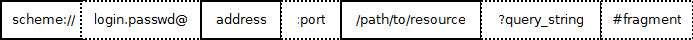
\includegraphics[width=0.9\columnwidth]{img/security/url-components}
		\caption{URL components. Optional components are indicated with dotted lines.}
		\label{fig:url-components}
	\end{center}
\end{figure}





\subsection{The HyperText Transfer Protocol}

Entering an URL into a browser navigation initiates an HTTP dialogue between browser and server. The server can be implemented in many different ways and essentially maps requests to responses [1]. The Hypertext Transfer Protocol (HTTP) is a stateless application-level request-response protocol that normally runs over TCP [1,2]. It is often used in combination with some mechanisms to track state [1] such as cookies and sessions, and often used in combination with authentication and/or secure communication extensions [1], like for example HTTPS.

HTTP request and response headers written in ASCII, and the HTTP contents are given in a MIME [2]. A general HTTP request consists out of a method, header and body, cf. \textbf{figure 2}. HTTP supports a variety of methods, but only two matter in practice, as shown in \textbf{table 1}. Other methods are for example DELETE, PUT, and HEAD [2]. HTTP request headers may take a several forms. Much of the metadata in an HTTP request header is security relevant [1].

\begin{lstlisting}[language=xml, caption=HTTP request., label=listing:http-request]
<METHOD> /path/to/resource?query_string HTTP/1.1
<header>*

<BODY>
\end{lstlisting}


\begin{table}[H]
	\caption{Part of the HTTP request API, adapted from \cite{Tanenbaum:2002:CN:572404}.}
	\label{tab:api:collections}
	\begin{tabular}{p{150px} | p{250px}}
		\textbf{Operation} & \textbf{Description} \\
		\hline
		\texttt{GET} 	& Read a web page. Intended for information retrieval Typically the body is empty. \\
		\texttt{POST} 	& Append to a web page. Intended for submitting information. Typically the body contains the submitted information. \\
		\hline
	\end{tabular}
\end{table}


\begin{table}[H]
	\caption{Some HTTP request message headers, adapted from \cite{Tanenbaum:2002:CN:572404}.}
	\label{tab:}
	\begin{tabular}{p{75px} | p{75px} | p{200px} }
		\textbf{Header} & \textbf{Type} 	& \textbf{Meaning} \\
		\hline
		Accept					& Request & The type of pages the client can handle. 							\\
		Accept-Charset	& Request & The character sets that are acceptable to the client. \\
		Host						& Request & The server's DNS name. 																\\
		Authorization		& Request & A list of the client's credentials. 									\\
		Referer					& Request & The previous URL from which the request came.					\\
		Cookie					& Request & Previously set cookie sent back to the server. 				\\
		\hline
	\end{tabular}
\end{table}


The general structure of an HTTP response is shown in \textbf{figure 3}. Similar to the request headers, response headers also contain security relevant metadata. Important HTTP response status codes are listed in \textbf{table 3}.

\begin{lstlisting}[language=xml, caption=HTTP response., label=listing:http-request]
HTTP/1.1 <STATUS CODE> <STATUS MESSAGE>
<header>*

<BODY>
\end{lstlisting}

\begin{table}[H]
	\caption{Status code response groups, adapted from \cite{Tanenbaum:2002:CN:572404}.}
	\label{tab:}
	\begin{tabular}{p{75px} | p{75px} | p{200px} }
		\textbf{Code} & \textbf{Meaning} 	& \textbf{Examples} \\
		\hline
		$1xx$	& Information 	& $100$ = server agrees to handle client's request. 		\\
		$2xx$	& Success 			& $200$ = request succeeded; $204$ = no content present \\
		$3xx$	& Redirection 	& $301$ = page moved; $304$ = cached page still valid 	\\
		$4xx$	& Client error	& $403$ = forbidden page; $404$ = page not found 				\\
		$5xx$	& Server error	& $500$ = interal server error; $503$ = try again later \\
		\hline
	\end{tabular}
\end{table}



\begin{table}[H]
	\caption{Some HTTP response message headers, adapted from \cite{Tanenbaum:2002:CN:572404}.}
	\label{tab:}
	\begin{tabular}{p{75px} | p{75px} | p{200px} }
		\textbf{Header} & \textbf{Type} & \textbf{Meaning} \\
		\hline
		Set-Cookie				& Response & Cookie for the client to store. 							\\
		Server						& Response & Information about the server. 								\\
		Content-encoding	& Response & How the content is encoded, e.g. gzip. 			\\
		Content-type			& Response & The page's MIME type. 												\\
		Last-modified			& Response & The last time the page was changed. 					\\
		Location					& Response & Tells the client where to send its request. 	\\
		\hline
	\end{tabular}
\end{table}


\subsubsection{HTTP Secure}

The HTTP protocol itself does not provide secure communication, but the HTTP Secure (HTTPS) protocol scheme runs HTTP on top of SSL/TLS, a standardized transport layer security protocol [1]. Secure Sockets Layer (SSL) is a software security package built in in pretty much all modern browsers. Via the SSL protocol, a secure connection is set up between two sockets. It handles compression and encryption [2]. SSL/TLS is very configurable, and the security guarantees it offers depend on configuration [1]:
\begin{itemize}
	\item Usually: communication integrity and confidentiality;
	\item Sometimes: server authentication;
	\item Every now and then: client authentication;
\end{itemize}


\subsubsection{Sessions on top of HTTP}

In order to group requests from the same user, a server creates a session-id and ensures that this session-id is sent with every request, by means of either Cookies, or embedding the id in URL's and/or form fields.

Cookies are small pieces of data that are stored by the server in the client's browser as key-value pairs using the Set-cookie header. In subsequent requests by the client, this cookie is automatically sent back to the web server using the Cookie header [1]. The cookie mechanism allows websites to build and maintain state over the otherwise stateless HTTP protocol [3]. The server can control various aspects, such as [1,2]:
\begin{itemize}
	\item Expiration date (Expires field);
	\item Domain and path scope of the cookie (Path field);
	\item Security aspects: limit to https, no access from scripts (Secure field).
\end{itemize}

\textbf{Listing 1} shows how you could set up a mechanism to keep track of a user as he/she is browsing your website using parameters in the query string. This is not ideal, but it works for simple applications.

\begin{lstlisting}[language=php, caption=Example of how state can be maintained using URLs and PHP., label=listing:]
<?php
$user = $_GET['user'];
if (empty($user)) {
	$user = $controller->get_new_user_id();
}
?>
<a href="http://www.somewebsite.com/nextpage?user=<?php echo $user; ?>">
	Next page
</a>
\end{lstlisting}


Web sessions are fragile from the point of view of security. Prof. Frank Piessens discusses a number of vulnerabilities in his slides [1], as discussed further in the text.


\subsubsection{HTTP Authentication}

Basic HTTP authentication can be done by including username and password in the Authorization request header, cf. \textbf{table 2}. Users are usually authenticated at application-level through a form where username and password are transmitted over HTTPS and validated by server application.

Single-Sign-On use federated identies to support a single user-id/password combination for multiple web applications.



\subsection{HyperText Markup Language}

HyperText markup language (HTML) is a markup language for creating web pages and other information that can be displayed in a web browser. It usually contains or contains references to CSS and JavaScript code. \textbf{Listing 2} shows an example of a simple HTML web page.

\begin{lstlisting}[language=java, caption=An example HTML web page., label=listing:]
<!DOCTYPE html PUBLIC "-//W3C//DTD XHTML 1.0 Transitional//EN" "http://www.w3.org/TR/xhtml1/DTD/xhtml1-transitional.dtd">
<html xmlns="http://www.w3.org/1999/xhtml" xml:lang="en" lang="en">
    <head>
        <meta http-equiv="Content-Type" content="text/html; charset=UTF-8"/>
        <title>EXAMPLE</title>
        <meta name="description" content="Example web page"/>
        <meta name="keywords" content="html example" />
    </head>
    <body>
        <div>
            <p>This is an example HTML web page.</p>
        </div>
    </body>
</html>
\end{lstlisting}

The formatting commands in HTML correspond to a set of tags with associated attributes [2]. These tags and attributes can be used in HTML to include pointers to, and content from other sites, e.g. [1]:
\begin{itemize}
	\item The <href> attribute: clickable link to a URL
	\item The <img> tag: links to an image that is automatically retrieved and displayed
	\item The <script> tag: can link to a script that is automatically  downloaded and executed
\end{itemize}


\subsection{JavaScript}

JavaScript is a client side scripting language. It is considered a dangerous aspect of websites as it allows to run foreign code on a client machine [2].

\begin{lstlisting}[language=java, caption=A simple JavaScript script to welcome a user., label=listing:]
var name = prompt("Please enter your name", "your name");
alert("Hello " + name + "!");
\end{lstlisting}